\chapterimage{chapter_head_1.pdf} % Chapter heading image
\chapter{일기도 그리기}

\section{일기도란}\index{일기도란}

\subsection{일기도(synoptic chart)}\index{일기도}

일정 시각의 넓은 지역에 걸친 기상 상태를 기호나 등치선으로 표현한 일기도를 말한다. 최초의 일기도는 독일의 천문학자, 수학자, 공학자인 하인리히 브란데스(Heinrich Wilhelm Brandes, 1777∼1834)에 의해서 작성되었다. 1821년 12월 24일과 25일 그리고 1823년 2월 2일과 3일에 작성된 브란데스의 일기도는 그의 저서 『기압의 급격한 변화에 관하여(On Rapid Changes in Pressure)』에 수록되어 1826년에 출판되었다.
일기도의 목적은 대기 중의 기상 상태를 입체적으로 관측하는 것이다. 이것을 이용하여 각 지역의 일기를 알 수 있으며, 연속된 일기도를 통해 앞으로의 일기를 예상할 수 있다. 정확한 일기 예보를 위해서는 지상으로부터 상층까지 그리고 시간적, 공간적으로 많은 일기도가 필요하다. 일기도에는 지상 일기도, 상층 일기도 그리고 보조선도 등이 있다.

%[네이버 지식백과] 종관일기도 [綜觀日氣圖, synoptic chart] (지구과학사전, 2009. 8. 30., 북스힐)
국제 협정에 의해 전 지구 상에서 동시에 지상 관측이 행해지는 시각으로 GMT(Greenwich Mean Time; 그리니치 표준시)가 사용되는데, 1994년부터는 UTC(Universal Time Coordinated; 협정 세계시)시각으로 사용되고 있다. 보통 일기도는 00:00로부터 매 3시간 간격으로 1일 8회 생산된다.


\subsubsection{일기도의 종류(규모에 따라)}\index{일기도의 종류}

\begin{itemize}
	\item 북반구 일기도 : 대규모의 기압계, 전선, 온도 분포의 개요 분석 등 장기 예보용 일기도이다.
	\item 아시아 태평양 일기도 : 장기 예보용 일기도이다.
	\item 극동 일기도 : 우리 나라 주변의 상세한 일기 분포 및 일기 파악에 사용된다.
	\item 국지 일기도 : 뇌우, 강수량 등의 상세한 분포 조사와 세밀한 기압 배치 및 국지 기상 파악에 사용된다.
\end{itemize}

\subsubsection{일기도가 제공하는 정보}\index{일기도가 제공하는 정보}
\begin{itemize}
	\item 바람의 강도와 방향
	\item 바람이 수렴하고 발산하는 지역, 즉 악기상이 발달하는 지역
	\item 상세한 구름의 구조와 분포
	\item 주요 기상이 나타나는 지역
	\item 국지 기상 효과들
	\item 각 기압계의 상세한 이동
\end{itemize}


\subsection{지도 투영법(map projection)}

구형인 지구 표면 상의 점을 평면상에 표시하는 방법으로 지구 상의 경위도선을 평면 상에 투영하는 것이다. 지구 표면을 거리, 면적, 모양 등 어느 면에서도 전혀 왜곡이 없도록 전개한다는 것은 불가능하다.

%[네이버 지식백과] 지도투영법 [map projection, 地圖投影法] (광물자원용어사전, 2010. 12., 한국광물자원공사)

%Previously we noted that the earth is really big. Not only is it big, but it is a big round spherical shape called a spheroid. A globe is a very common and very good representation of the three-dimensional, spheroid earth. One of the problems with globes, however, is that they are not very portable (i.e., you cannot fold a globe and put in it in your pocket), and their small scale makes them of limited practical use (i.e., geographic detail is sacrificed). To overcome these issues, it is necessary to transform the three-dimensional shape of the earth to a two-dimensional surface like a flat piece of paper, computer screen, or mobile device display in order to obtain more useful map forms and map scales. Enter the map projection.

%Map projections refer to the methods and procedures that are used to transform the spherical three-dimensional earth into two-dimensional planar surfaces. Specifically, map projections are mathematical formulas that are used to translate latitude and longitude on the surface of the earth to x and y coordinates on a plane. Since there are an infinite number of ways this translation can be performed, there are an infinite number of map projections. The mathematics behind map projections are beyond the scope of this introductory overview (but see Robinson et al. 1995; Muehrcke and Muehrcke 1998),Muehrcke, P., and J. Muehrcke. 1998. Map Use. Madison, WI: JP Publications. and for simplicity, the following discussion focuses on describing types of map projections, the distortions inherent to map projections, and the selection of appropriate map projections.

%To illustrate the concept of a map projection, imagine that we place a light bulb in the center of a translucent globe. On the globe are outlines of the continents and the lines of longitude and latitude called the graticule. When we turn the light bulb on, the outline of the continents and the graticule will be “projected” as shadows on the wall, ceiling, or any other nearby surface. This is what is meant by map “projection.”

%Within the realm of maps and mapping, there are three surfaces used for map projections (i.e., surfaces on which we project the shadows of the graticule). These surfaces are the plane, the cylinder, and the cone. Referring again to the previous example of a light bulb in the center of a globe, note that during the projection process, we can situate each surface in any number of ways. For example, surfaces can be tangential to the globe along the equator or poles, they can pass through or intersect the surface, and they can be oriented at any number of angles.

\ref{fig:map_projection} \과 같이 광원의 위치와 빛이 투영되는 스크린의 위치와 모양을 달리하면 여러 방법으로 지구를 평면에 투영할 수 있다. 원통 도법은 지구의 표면을 원통으로 투영하여 그리는 것으로 도법으로 그리면 경선과 위선이 직각으로 교차한다. 원뿔 도법은 지구의 어떤 위선에 원뿔면을 접하게 하고 그 위에 투영된 지구 표면의 형태를 그리는 것으로 지구의 일부분만 나타낼 수 있다. 평면 도법은 평면에 투영하여 그리는 것으로 지구의 반구 부분만 나타낼 수 있다.

\begin{figure}[h]
	\centering
	\includegraphics[width=0.95\linewidth]{22Weather_forecasting/images/projection_families}
	\caption{지도 투영법}
	\label{fig:map_projection}
	 %%http://docs.qgis.org/2.0/en/_images/projection_families.png
\end{figure}

\subsection{일기도용 지도 투영법}
일기도를 그리는 지도는 세계 각지에서 관측된 기상관측자료들의 기입을 위해서는 연속된 등치선(isopleth)들을 그릴 수 있도록 해당대륙이나 대양이 분열되지 않는 지도여야 한다.

\subsubsection{극 평사 도법(polar stereographic projection)}
북반구 또는 남반구를 위도 60$^{\circ}$ 를 표준 위도선으로 절단시켰다고 생각하는 가상 평면 상에 반대쪽 극(極)에 광원(光源)을 놓고 투영한다. 이 투영법으로 한쪽 반구를 전부 나타낼 수 있어서 반구 중의 대륙이나 대양을 나타내는 일기도에 적합하다. 표준 위도 부근에서는 그 면적이 축척에 비슷하나 표준 위도로부터 멀어질수록 오차가 커진다. 적합한 축척은 1:1500만, 1:2000만, 1:3000만 정도가 좋다.

\subsubsection{람베르트 원뿔 도법(Lambert conformal conic projection)}
한쪽 반구를 위도 10$^{\circ}$와 40$^{\circ}$ 또는 30$^{\circ}$와 60$^{\circ}$의 표준 위도선을 절단하는 원추면에 지구 중심에 있는 광원을 투영시켜 만든 지도이다. 이 지도는 중위도 지방의 한 대륙이나 대양 정도의 크기를 나타내는 일기도를 만들 때 적당하다. 이때 축척은 보통 1:750만 - 1:2000만 정도이다.

%%%
%%%\begin{figure}[h!]\center
%%%	\centering
%%% \includegraphics[width=0.8\linewidth]{22Weather_forecasting/images/1008px-Lambert_conformal_conic}
%%%	\caption{람베르트 원추도법(Lambert conformal conic projection)}
%%%	\label{fig:1008px-Lambert_conformal_conic}
%%%	%https://upload.wikimedia.org/wikipedia/commons/thumb/2/24/Lambert_conformal_conic.svg/1008px-Lambert_conformal_conic.svg.png
%%%\end{figure}


%%%\begin{figure}[!htb]\centering
%%%	\begin{minipage}{0.49\textwidth}
%%%		\frame{\includegraphics[width=0.45\linewidth]{22Weather_forecasting/images/polar_stereographic_projection}}
%%%		\caption{극평사도법}
%%%		\label{fig:polar_stereographic_projection}
%%%	\end{minipage}
%%%	\begin {minipage}{0.49\textwidth}
%%%	\frame{\includegraphics[width=0.45\linewidth]{22Weather_forecasting/images/Lambert_conformal_conic_projection}}
%%%		\caption{람베르트 원추도법}
%%%		\label{fig:Lambert_conformal_conic_projection}
%%%\end{minipage}
%%%\end{figure}


\subsubsection{메르카토르 원통 도법(Mercator projection)}
남북반구의 위도 23.5$^{\circ}$를 표준 위도선으로 하여 이를 절단하도록 씌운 원통 면에다 지구 중심에 광원(光源)을 놓아 투영하는 지도. 단점은 극지방의 면적이 과대하게 커 보이지만 장점으로 적도부근 지방에서는 비교적 정확하고 방위가 정확하다. 또한 지구의 대부분을 나타낼 수 있어 전구 혹은 적도 부근의 일기도용 지도에 적합하다. 1:3000만 또는 1:6000만 축척이 좋다.

%%일기도 [weather chart] (기상백과, 기상청)

\section{일기도의 종류}\index{일기도의 종류}
여기서는 현재 기상청(www.kma.go.kr)에서 제공하는 일기도를 기준으로 설명한다.

\subsection{지상 일기도}\index{지상 일기도}
 지상 일기도는 기상 관측을 근거로 하여 컴퓨터가 작성하고 예보관이 세밀하게 수작업으로 보완, 수정하여 작성한 일기도 이다. 고기압과 저기압의 분포에 따른 날씨 분포를 알아내는데 이용한다.

\subsubsection{지상03}\index{지상03}
지상03 일기도는 00 UTC 기준 3 시간 간격 (00, 03, 06, 09, 12, 15, 18, 21 UTC) 으로 작성하는데, 각 관측소의 지상 기상 관측값을 볼 수 있다. 1,000 hPa 기준 2 hPa 간격으로 등압선을 그린다. 

%%#\begin{figure}[h]\center
%%#	\centering
%%#	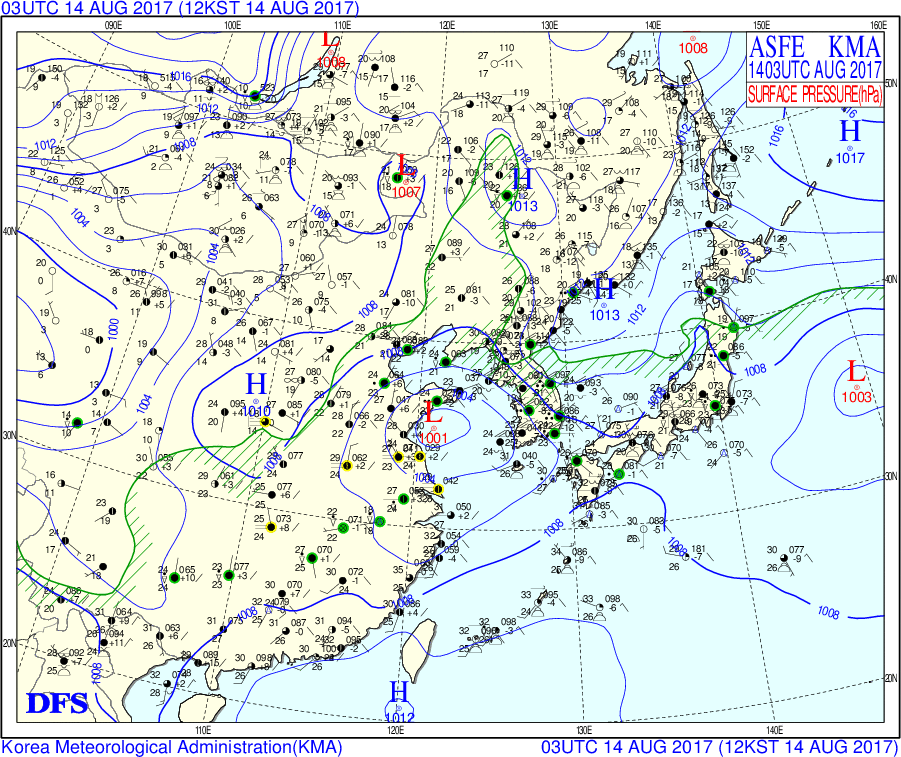
\includegraphics[width=0.97\linewidth]{22Weather_forecasting/images/sfc3_2017081403}
%%#	\caption{지상03 일기도(www.kma.go.kr)}
%%#	\label{fig:draw-weathermapsurf03}
%%#\end{figure}

\subsubsection{지상12}\index{지상12}
지상12 일기도는 00 UTC 기준 12시간 간격 (00, 12 UTC)으로 전 세계 동시에 작성한다. 각 관측소의 지상 기상 관측값을 볼 수 있고, 1,000 hPa 기준 4 hPa 간격으로 등압선을 그린다. 

\begin{figure}[p]\centering
	\begin{minipage}{0.97\textwidth}
	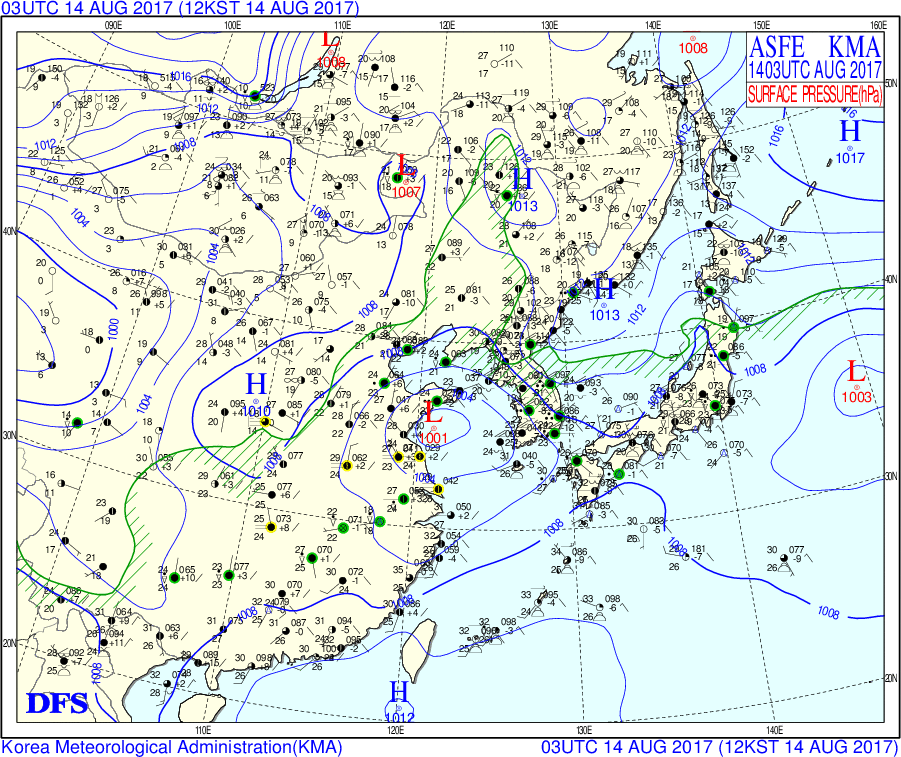
\includegraphics[width=0.97\linewidth]{22Weather_forecasting/images/sfc3_2017081403}
	\caption{지상03 일기도(www.kma.go.kr)}
\label{fig:draw-weathermapsurf03}
	\end{minipage}
	\begin{minipage}{0.97\textwidth}
	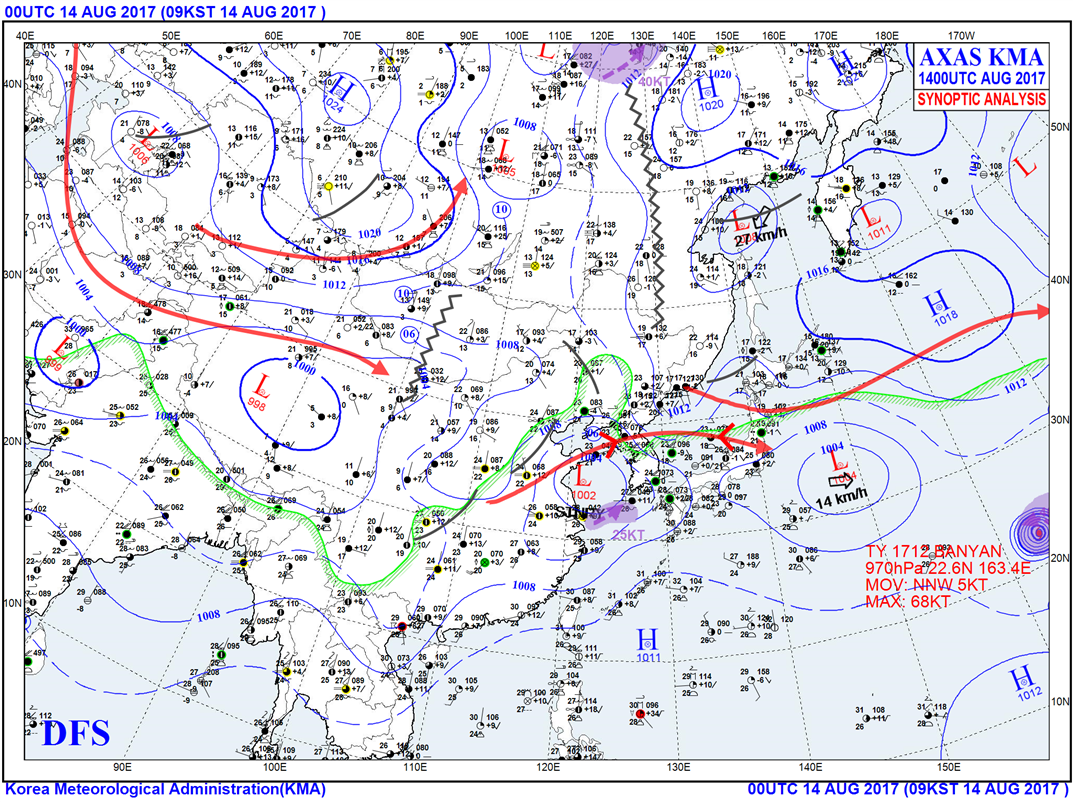
\includegraphics[width=0.97\linewidth]{22Weather_forecasting/images/surf_2017081400}
		\caption{지상12 일기도(www.kma.go.kr)}
		\label{fig:draw-weathermapsurf12}
	\end{minipage}
\end{figure}

\newpage
\subsection{상층 일기도}\index{상층 일기도}

상층의 등압면 고도, 기온, 풍속, 습도 등의 분포도를 말하며 고층 일기도라고도 한다. 고층의 일기 상태를 지상 일기도와 같이 평면적으로 나타낸 일기도이다. 기상청에서는 강수량 및 하층 대기의 기온 변화 예상에 필요한 925 hPa, 850 hPa, 700 hPa 일기도와 중층 대기에 대규모적인 기류 분석에 쓰이는 500 hPa 일기도, 대류권과 성층권 경계 부근의 제트기류 분석 등에 쓰이는 300 hPa (여름철에는 200 hPa), 항공기류 분석을 위해 100 hPa을 하루 두 번 (09시, 21시) 분석한다. 상층의 고기압과 저기압의 분포, 기단(기온) 분포, 건습(습도) 분포 등을 알아내는 데 이용된다.
%[네이버 지식백과] 상층일기도 [upper-air chart] (기상백과, 기상청)

\subsubsection{925 hPa 면 (810 m)}\index{925 hPa 면 (810 m)}
대류권의 최하층인 평균 810 m 높이의 기상 상황을 나타내는 상층 일기도이다. 각 관측소의 925 hPa 면의 상층 기상 관측값을 810 m기준 30 m 간격 등고선(청색 실선)과 3℃간격 등온선(적색 파선), 습윤 구역(노점 편차 < 2℃: 녹색 칠)로 나타낸다. 

\subsubsection{850 hPa 면 (1,500 m)}\index{850 hPa 면 (1,500 m)}
대기의 하층에 해당하는 지상 평균 1,500 m 높이의 상층 일기도로 지상 일기도와 대응시켜 사용되며, 전선 분석에 이용된다. 각 관측소의 850 hPa 면의 상층 기상 관측값을 1,500m기준 30m 간격 등고선(청색 실선)과 0℃ 기준 3℃간격 등온선(적색 파선), 습윤 구역(노점 편차 < 3℃: 녹색칠)을 나타낸다.

\subsubsection{700 hPa 면 (3,000 m)}\index{700 hPa 면 (3,000 m)}
대기의 하층에 해당하는 지상 평균 3,000 m 높이의 대류권 하층을 대표하는 고도의 상층 일기도로 수증기 분석에 적합하다. 각 관측소의 700 hPa 면의 상층 기상 관측값을 3,000 m 기준 60 m 간격 등고선(청색 실선)과 0℃ 기준 5℃ 간격 등온선(적색 파선), 습윤 구역(노점 편차 < 4℃: 녹색칠)을 나타낸다. 

\subsubsection{500 hPa 면 (5,580 m)}\index{500 hPa 면 (5,580 m)}
대기의 하층에 해당하는 지상 평균 5,580 m 높이의 대류권 중층(비발산 고도)으로 광범위한 대기 환류 조사에 적합하다. 각 관측소의 500 hPa 면의 상층 기상 관측값을 5,580 m 기준 60 m 간격 등고선(청색 실선)과 0℃ 기준 5℃ 간격 등온선(적색 파선) 나타낸다. 

\subsubsection{300 hPa 면 (9,180 m)}\index{300 hPa 면 (9,180 m)}
대류권의 상중층인 지상 평균 9,180 m 높이의 상층 일기도로 편서풍이 강하게 나타나며 제트류의 해석에 편리하다. 각 관측소의 300 hPa 면의 상층 기상 관측값을 9,180 m 기준 120 m 간격 등고선(청색 실선)과 0℃ 기준 5℃ 간격 등온선(적색 파선), 75 kt 기준 25 kt 간격의 등풍속선(녹색 실선), 강풍 구역(75 kts 이상 :  녹색점 집합), 제트기류 축(적색 띠 화살표)을 나타낸다. 

\subsubsection{200 hPa 면 (11,760 m)}\index{200 hPa 면 (11,760 m)}
대류권의 상층인 지상 평균 11,760 m 높이의 상층 일기도로 300hPa과 비슷하며 항공기에 대한 비행 정보 제공에 이용된다. 각 관측소의 200 hPa 면의 상층 기상 관측값을 11,760 m 기준 120 m 간격 등고선(청색 실선)과 0℃ 기준 5℃ 간격 등온선(적색 파선), 75 kt 기준 25 kt 간격의 등풍속선(녹색 실선), 강풍 구역(75 kts 이상 :  녹색점 집합), 제트기류 축(적색 띠 화살표)을 나타낸다. 

\subsubsection{100 hPa 면 (16,200 m)}\index{100 hPa 면 (16,200 m)}
대류권의 상층인 지상 평균 16,200 m 높이의 상층 일기도로 편서풍이 강하게 나타나며 제트류의 해석에 편리하다. 각 관측소의 100 hPa 면의 상층 기상 관측값을 16,200 m 기준 120 m 간격 등고선(청색 실선)과 0℃ 기준 5℃ 간격 등온선(적색 파선), 75 kt 기준 25 kt 간격의 등풍속선(녹색 실선), 강풍 구역(75 kts 이상 :  녹색점 집합), 제트기류 축(적색 띠 화살표)을 나타낸다. 

\begin{figure}[p]\centering
	\begin{minipage}{0.97\textwidth}
	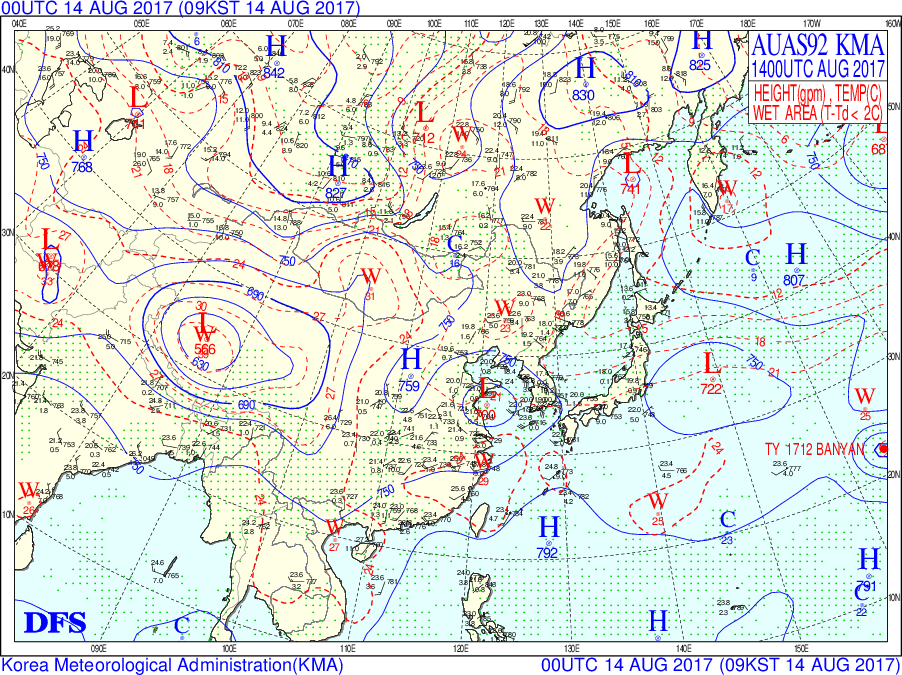
\includegraphics[width=0.97\linewidth]{22Weather_forecasting/images/up92_2017081400}
		\caption{925hPa 상층 일기도(www.kma.go.kr)}
		\label{fig:draw-weathermapsurf92}
	\end{minipage}
	\begin{minipage}{0.97\textwidth}
	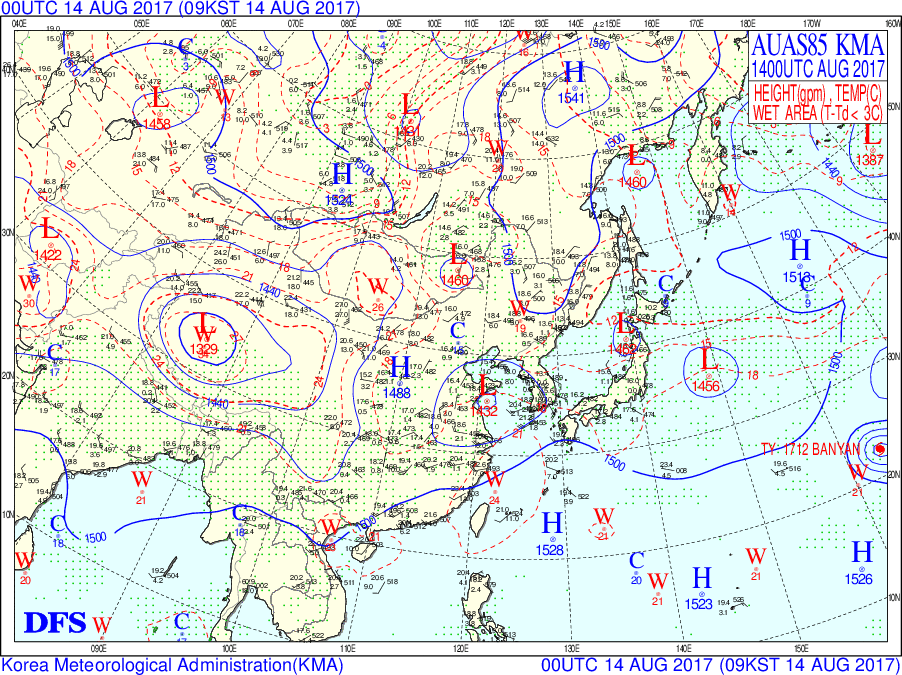
\includegraphics[width=0.97\linewidth]{22Weather_forecasting/images/up85_2017081400}
		\caption{850hPa 상층 일기도(www.kma.go.kr)}
		\label{fig:draw-weathermapsurf85}
	\end{minipage}
\end{figure}

\begin{figure}[p]\centering
	\begin{minipage}{0.97\textwidth}
	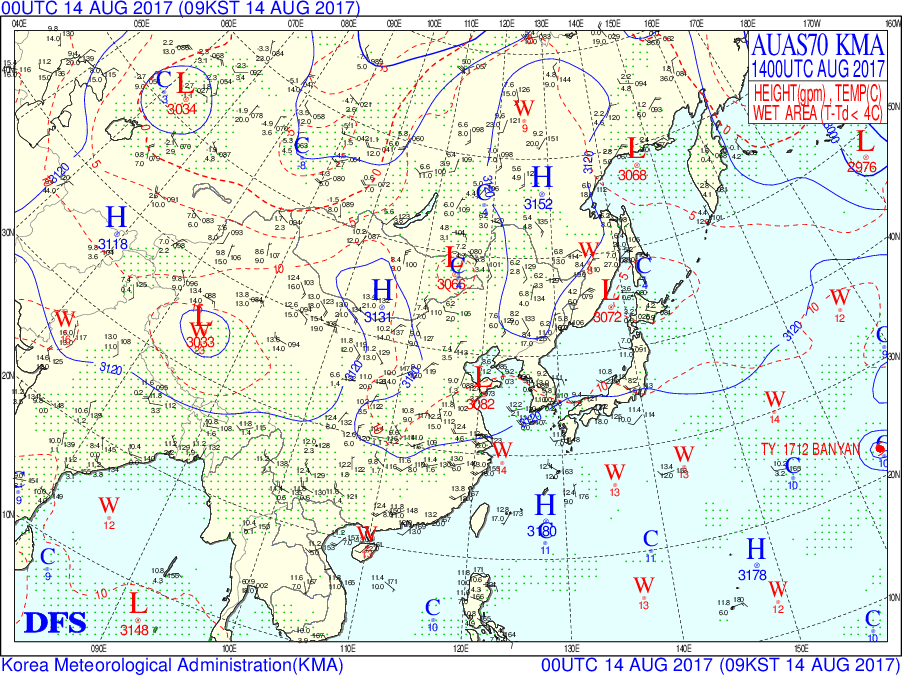
\includegraphics[width=0.97\linewidth]{22Weather_forecasting/images/up70_2017081400}
		\caption{700hPa 상층 일기도(www.kma.go.kr)}
		\label{fig:draw-weathermapsurf70}
	\end{minipage}
	\begin{minipage}{0.97\textwidth}
	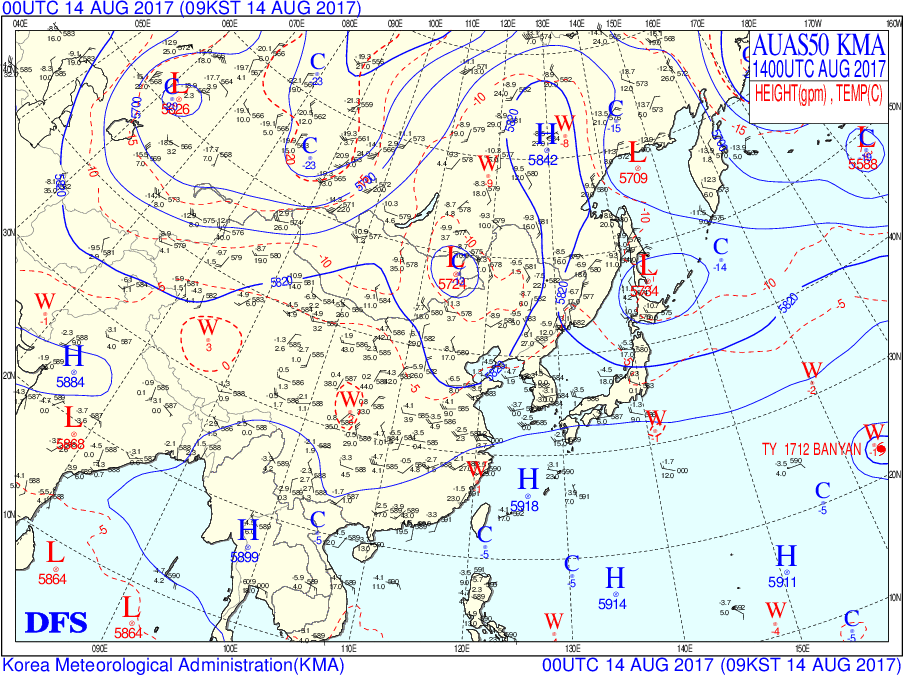
\includegraphics[width=0.97\linewidth]{22Weather_forecasting/images/up50_2017081400}
		\caption{500hPa 상층 일기도(www.kma.go.kr)}
		\label{fig:draw-weathermapsurf50}
	\end{minipage}
\end{figure}

\begin{figure}[p]\centering
	\begin{minipage}{0.97\textwidth}
	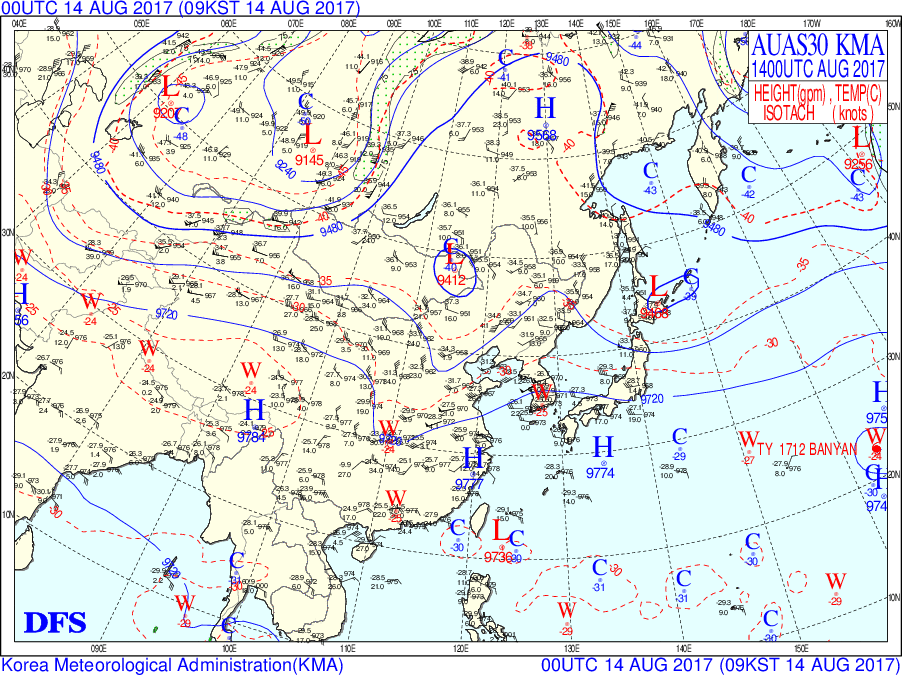
\includegraphics[width=0.97\linewidth]{22Weather_forecasting/images/up30_2017081400}
		\caption{300hPa 상층 일기도(www.kma.go.kr)}
		\label{fig:draw-weathermapsurf30}
	\end{minipage}
	\begin{minipage}{0.97\textwidth}
	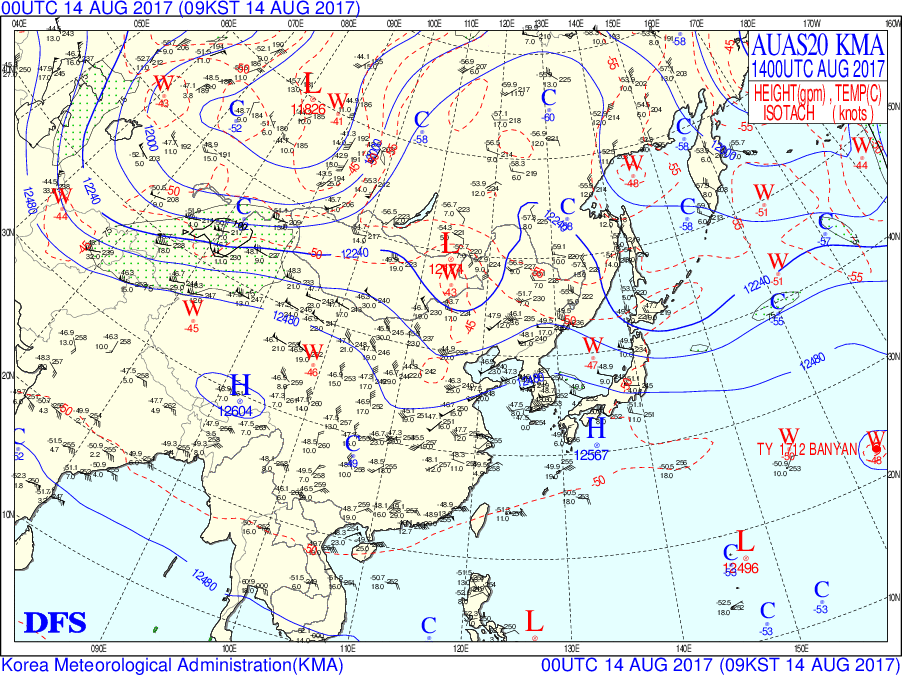
\includegraphics[width=0.97\linewidth]{22Weather_forecasting/images/up20_2017081400}
		\caption{200hPa 상층 일기도(www.kma.go.kr)}
		\label{fig:draw-weathermapsurf20}
	\end{minipage}
\end{figure}

\begin{figure}[h]\center
	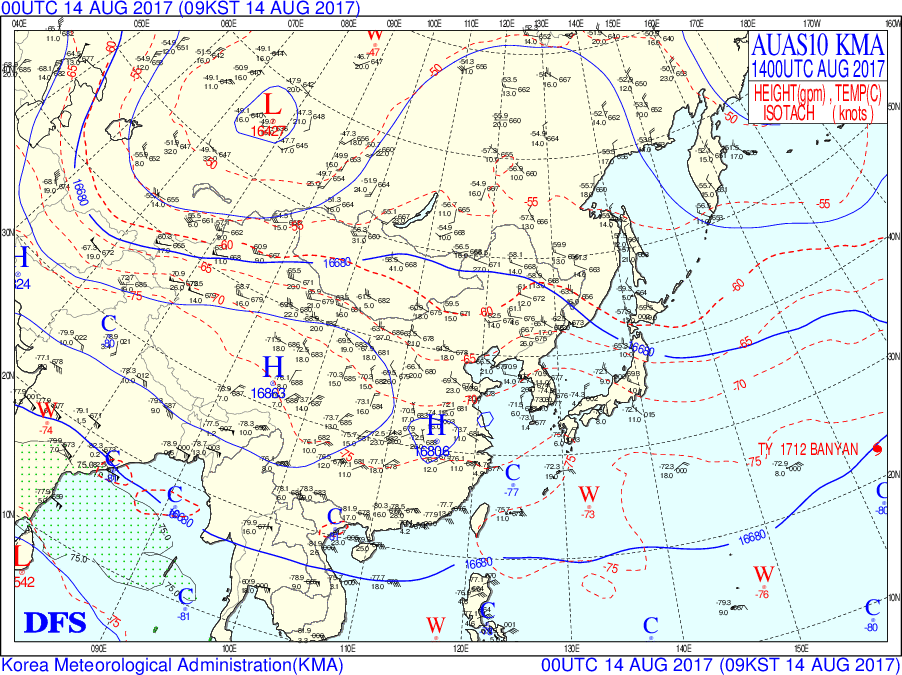
\includegraphics[width=0.97\linewidth]{22Weather_forecasting/images/up10_2017081400}
	\caption{100hPa 상층 일기도(www.kma.go.kr)}
	\label{fig:draw-weathermapsurf10}
\end{figure}


	

%%#\begin{itemize}
%%#	\item 925hPa면 일기도(810m) : 지상 일기도와 대응시켜 사용되며, 전선 분석에 이용된다.
%%#	\item 850hPa면 일기도(1,500m) : 지상 일기도와 대응시켜 사용되며, 전선 분석에 이용된다.
%%#	\item 700hPa면 일기도(3,000m) : 대류권 하층을 대표로 하는 고도로 수증기 분석에 적합하다.
%%#	\item 500hPa면 일기도(5,580m) : 대류권 중층(비발산 고도)으로 광범위한 대기 환류 조사에 적합하다.
%%#	\item 300hPa면 일기도(9,180m) : 대류권 상층으로 편서풍이 강하게 나타난다. 제트류의 해석에 편리하다.
%%#	\item 200hPa면 일기도(11,760m) : 300hPa과 비슷하며 항공기에 대한 비행 정보 제공에 이용된다.
%%#\end{itemize}

%%#\begin{figure}[!htb]\centering
%%#	\begin{minipage}{0.49\textwidth}
%%#		\frame{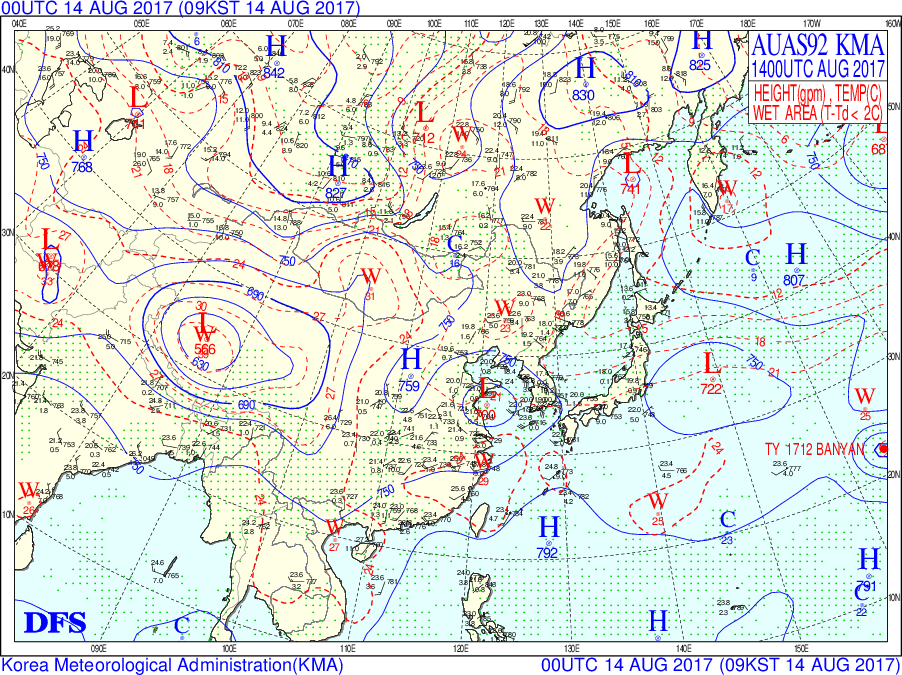
\includegraphics[width=0.95\linewidth]{22Weather_forecasting/images/up92_2017081400}}
%%#	\caption{925hPa 상층 일기도(www.kma.go.kr)}
%%#	\label{fig:draw-weathermapsurf92}
%%#	\end{minipage}
%%#	\begin {minipage}{0.49\textwidth}
%%#	\frame{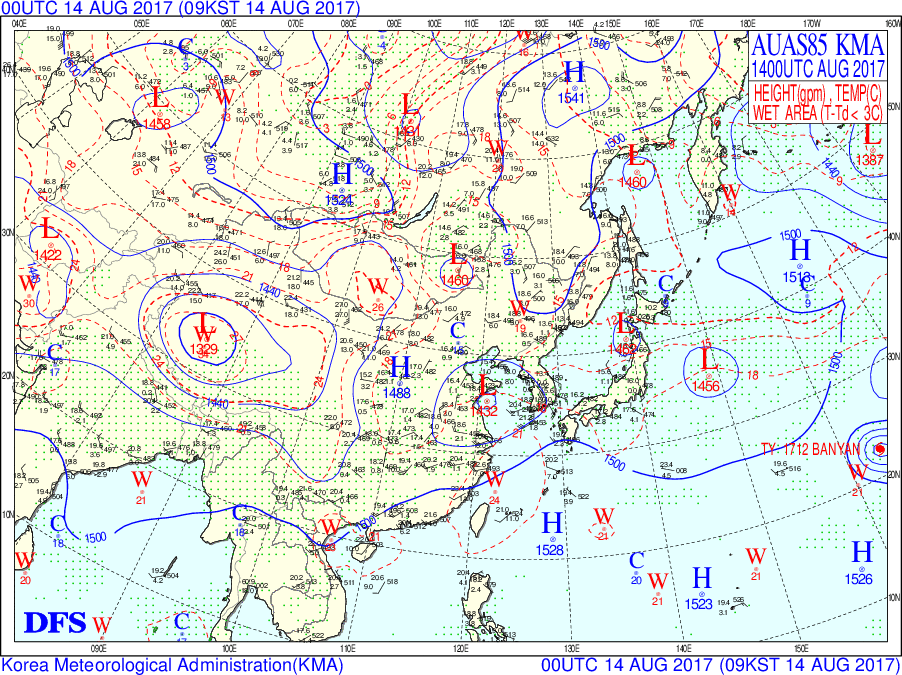
\includegraphics[width=0.95\linewidth]{22Weather_forecasting/images/up85_2017081400}}
%%#		\caption{850hPa 상층 일기도(www.kma.go.kr)}
%%#		\label{fig:draw-weathermapsurf85}
%%#	\end{minipage}
%%#\end{figure}


\newpage
\section{일기도 그리기}\index{일기도 그리기}

\subsection{기상 관측}\index{관측 자료 기입}
지상 혹은 상층 대기 상태를 요소별로 관측하는 것으로 관측 자료는 기상 예보 판단의 기본 요소가 된다.

\begin{itemize}
	\item 지상 관측: 운고, 운량, 운형, 시정, 기상 현상, 기압, 이슬점, 습도, 풍향, 풍속, 강수량, 적설량 및 기타 특수 현상을 목측 혹은 계기에 의해 관측하는 것을 말한다.
	\item 고층 기상 관측: 상층 고도별 풍향, 풍속, 기온, 이슬점 온도, 습도, 기압을 계기에 의해 측정한다.
	\item 상층풍 관측 : 상층의 고도별 풍향·풍속을 기구를 비양시켜 측정한다.
	\item 그 외에 레이더 관측, 항공기 관측, 위성 관측 등이 있다.
\end{itemize}


\subsection{기상 전문 기입}\index{기상 전문 기입}

WMO에서 지정한 각 지점에 주어진 시간의 기상 전문을 수신하여 일기도 각 지점에 기입해야 하는데, 일기도에 관측된 자료를 나타낼 때에는 \ref{fig:drawsymbols-1}\과 같이 정해진 형식으로 기입해야 한다. 단 예시에서 기온은 화씨임에 유의하라.

\begin{figure}[p]
	\centering
	\includegraphics[width=0.95\linewidth]{22Weather_forecasting/images/wxsymbol_print-1}
	\caption{일기도 기호 기입 형식(NOAA)}
	\label{fig:drawsymbols-1}
\end{figure}

\begin{figure}[p]
	\centering
	\includegraphics[width=0.95\linewidth]{22Weather_forecasting/images/wxsymbol_print-2}
	\caption{일기도 기호 기입 형식(NOAA)}
	\label{fig:drawsymbols-1}
\end{figure}

%%#\begin{figure}[p]
%%#	\centering
%%#	\includegraphics[width=0.95\linewidth]{22Weather_forecasting/images/wxsymbol_print-12}
%%#	\caption{일기도 기호 기입 형식(NOAA)}
%%#	\label{fig:drawsymbols}
%%#\end{figure}

\newpage
\subsection{등압선 그리는 방법}\index{등압선 그리는 방법}
일기도에서 가장 중요하게 다루는 선이 등압선이다. 등압선은 기압이 같은 지점을 연결한 선이다. 등압선을 그려 보면 고기압과 저기압의 위치, 전선 등을 가려 낼 수 있다. 이것은 마치 지도에 그려진 등고선의 분포 모양을 보고 산이나 골짜기를 판별하는 것과 유사하다. 

등압선은 다음과 같은 방법으로 그린다.
\begin{enumerate}
 \item 주어진 일기도에 기입된 각종 자료 중 구름의 양, 풍향, 풍속, 기압 등의 의미를 파악한다. 
 \item 해면 기압은 자연 상태에서 보통 1060 hPa을 넘지 않으므로, 첫자리 수가 0에서 5사이이면 10을, 6과 9사이 이면 9를 각각 앞에 붙여 계산한다.
 \item 일반적으로 등압선은 1000 hPa을 기준으로 ......, 992, 996, 1000, 1004, 1008, ...... 등 4 hPa 간격으로 그린다. 그러나 등압선 간의 폭이 너무 넓어 기압배치를 파악하기 어려울 때는 2 hPa 간격으로 파선을 그린다.
 \item 그리기 쉬운 곳(등압선이 조밀하지 않은 곳)부터 그려 나간다.
 \item 등압선은 중간에서 끊어지거나 없어지지 않는다.
 \item 관측값이 없는 경우는 내삽, 또는 외삽법의 원리로 \ref{fig:drawweathermap01}\과 같이 이웃하는 두 지점의 간격을 비례로 나누어서 부드럽고 매끈한 곡선으로 그린다.
 \item 한 선으로 연결되는 등압선은 양쪽 끝에 기압의 값을 기입하고, 폐곡선의 경우는 위쪽(북쪽) 중앙에 등압선을 끊고 값을 기입한다. 
 \item 저기압의 중심은 적색으로 L(low pressure), 고기압의 중심은 청색으로 H(high pressure)라고 표시한다.
\end{enumerate}

\begin{figure}[h]
	\centering
	\includegraphics[width=0.8\linewidth]{22Weather_forecasting/images/draw-weathermap01}
	\caption{등압선의 작도 방법}
	\label{fig:drawweathermap01}
\end{figure}

등압선을 그리고 나면 고기압과 저기압의 위치 및 이동경로, 기압과 고도의 변화경향, 전선의 발생 및 소멸과 이동, 날씨 변화, 대기의 수직 구조 등을 세밀히 분석하게 된다. 

전선의 위치를 찾는 방법은 다음과 같다.

\begin{enumerate}
 \item 전선은 기온, 이슬점, 풍향이 불연속을 이루므로 이들 값이 급변하는 지역을 찾는다.
 \item 전선 근처에서는 일반적으로 일기가 악화되므로 강수 등의 일기가 선상으로 나타날 경우 전선이 존재할 가능성이 높다. 
 \item 온난전선은 전면의 넓은 지역에서 강수 현상이 나타나고 후면에는 비교적 맑은 날씨를 이룬다. 한랭전선은 전면과 후면의 구별 없이 전선 상에서 비교적 좁은 지역에 강수 현상이 나타난다.
 \item 전선이 확인되면 \ref{fig:drawweathermap02}\와 같이 등압선이 휘도록 연결한다.
\end{enumerate}

\begin{figure}[h]
	\centering
	\includegraphics[width=0.8\linewidth]{22Weather_forecasting/images/draw-weathermap02}
	\caption{전선에서의 등압선}
	\label{fig:drawweathermap02}
\end{figure}

\newpage
\subsection{실습 에제}\index{실습 예제}
다음 일기도에 등압선을 그리고 고기압, 저기압의 위치 및 전선을 찾아 표시해 보자.

\subsubsection{전선이 그려진 경우}\index{전선이 그려진 경우}

\begin{figure}[h]\center
	\centering
	\includegraphics[width=1.0\linewidth]{22Weather_forecasting/images/isobar_ex01}
%	\caption{}
	\label{fig:isobar_ex01}
\end{figure}

\newpage
\subsubsection{전선이 한 개 있는 경우}\index{전선이 한개 있는 경우}

\begin{figure}[h]\center
	\centering
	\includegraphics[width=1.0\linewidth]{22Weather_forecasting/images/isobar_ex02}
	%	\caption{}
	\label{fig:isobar_ex02}
\end{figure}

\newpage
\subsubsection{전선이 두 개 있는 경우}\index{전선이 두 개 있는 경우}

\begin{figure}[h]\center
	\centering
	\includegraphics[width=1.0\linewidth]{22Weather_forecasting/images/isobar_ex03}
	%	\caption{}
	\label{fig:isobar_ex03}
\end{figure}

\newpage
\subsubsection{등압선 그리기}\index{등압선 그리기}

\begin{figure}[h]\center
	\centering
	\includegraphics[width=1.0\linewidth]{22Weather_forecasting/images/surf_pltstn_pbg_2004122400}
	\caption{등압선 그리기 예제}
	\label{fig:drawweathermap03}
\end{figure}

